\counterwithout{section}{chapter}

\section{Листинг кода}

Далее будут представлены листинги прерывания INT8h и процедуры sub\_2

\lstinputlisting[style={asm}, caption={Листинг прерывания INT 8h}]{../../src/INT8.LST}
\lstinputlisting[style={asm}, caption={Листинг процедуры sub\_2}]{../../src/SUB.LST}

\section{Схемы алгоритмов}

\begin{figure}[h!]
	\begin{center}
		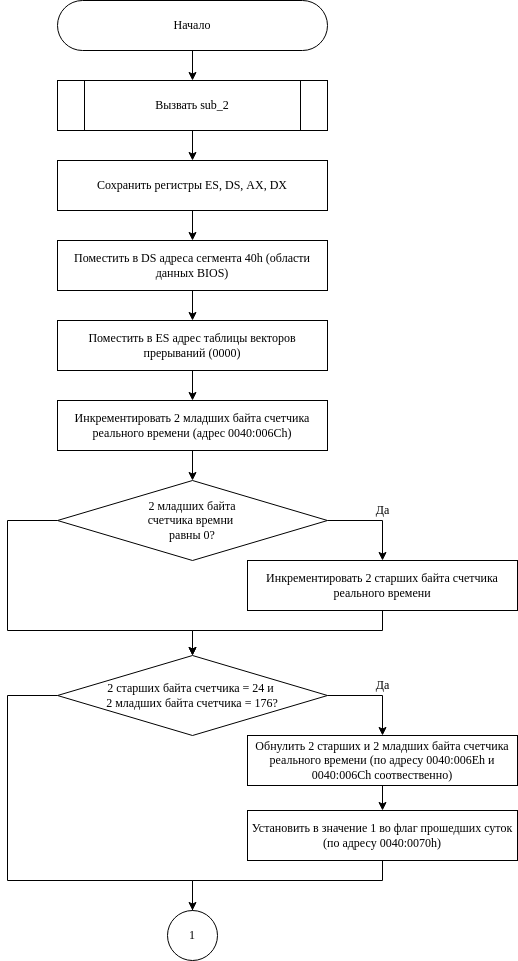
\includegraphics[scale=0.6]{../../INT8.drawio.png}
		\caption{Схема алгоритма прерывания INT 8h}
	\end{center}
\end{figure}

\begin{figure}[h!]
	\begin{center}
		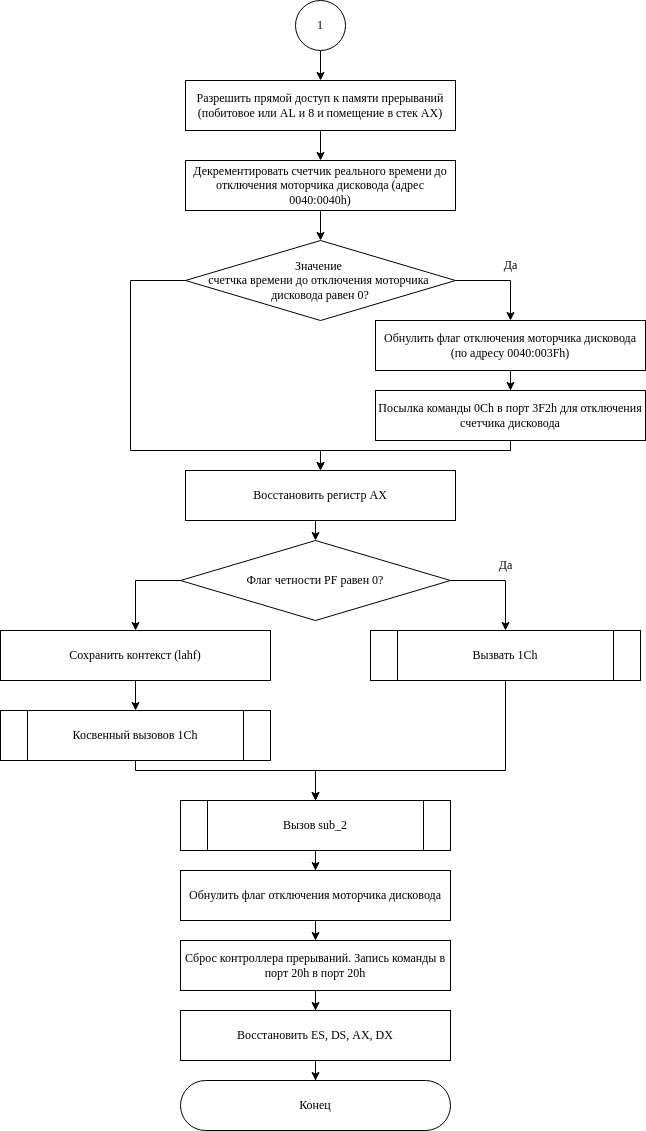
\includegraphics[scale=0.6]{../../INT8_END.drawio.png}
		\caption{Схема алгоритма прерывания INT 8h}
	\end{center}
\end{figure}

\begin{figure}[h!]
	\begin{center}
		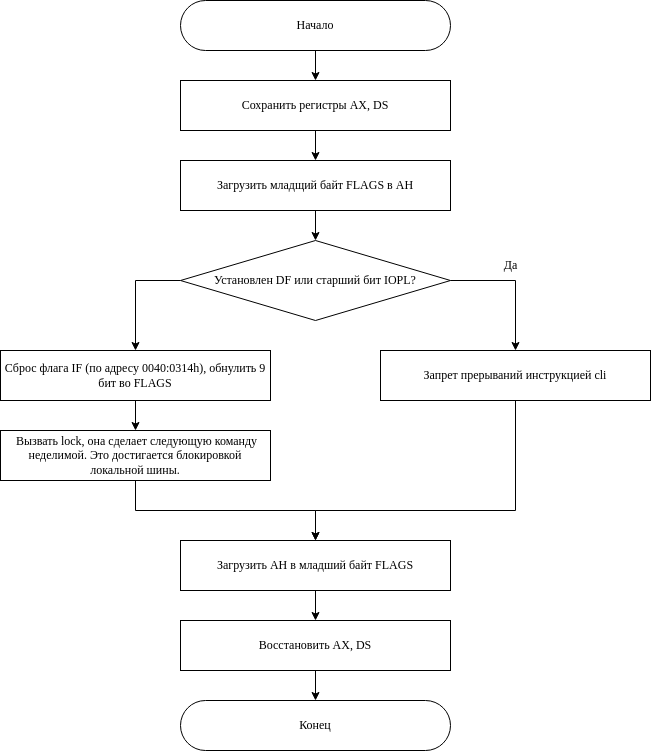
\includegraphics[scale=0.6]{../../SUB2.drawio.png}
		\caption{Схема алгоритма процедуры SUB 2}
	\end{center}
\end{figure}